%!TEX root=main.tex

\section{Introduction} \label{sec:intro}
For autonomous vehicles to drive fast and safe, it is important for the vehicles to correctly predict the intent (i.e., path prediction) of pedestrians, bicyclists, and drivers around them (\cref{fig:overview}). 
Previous works have attempted to predict intent of pedestrians and drivers. They have showed promising directions toward correctly estimating human intent, but the problem of correctly predicting the intent still remains challenging~\cite{Alahi2016, Morris2011}. 
On the other hand, humans excel at the task to estimate pedestrian and driver intent~\cite{Keller2014}. 
They exploit their intuitive understanding of physics~\cite{Battaglia2013} and hidden variables that describe human intent. Hidden variables can be the pedestrian's hidden goal, level of distraction, repulsiveness and attraction to other pedestrians or many more~\cite{Helbing1998}. Humans can infer these parameters for example from observing the body pose, gaze direction, mimic and observation of obstacles in the environment.

This project aims to understand human intent with computational models, such as the hidden Markov model (HMM) and a neural network model. The pedestrian prediction task is simplified as collision prediction task to allow for comparison.

First, a human is tasked to predict if two pedestrians are going to collide, given a simulated video sequence. Second, an HMM is learned to infer collision probability from the same data and the prior is adapted to better imitate the human predictive capabilities. Third, an ensemble of neural network is trained on a bigger dataset and it's predictive mean and uncertainty is compared against the human decision making. 

This project analyses the capability of humans to predict pedestrian intent and evaluates an HMM and Neural Network model to copy this capability. The HMM's posterior is adapted to closely resemble human decision making and indicates that humans strongly rely on the heading and euclidean distance information to predict collisions. The neural network model was trained to predict collision probability. Additionally, we use an ensemble of neural networks to estimate uncertainty. The neural network model achieves the Pearson correlation of $0.69$ between a human data and model's prediction. As we show, the neural network model is less capable to perform than humans to predict novel behavior, but interestingly is uncertain for the same region as humans are.

All source code and results can be found at 
$https://github.com/dkkim93/9.66\_collision\_final\_project$.

\begin{figure}[t]
  \centering
  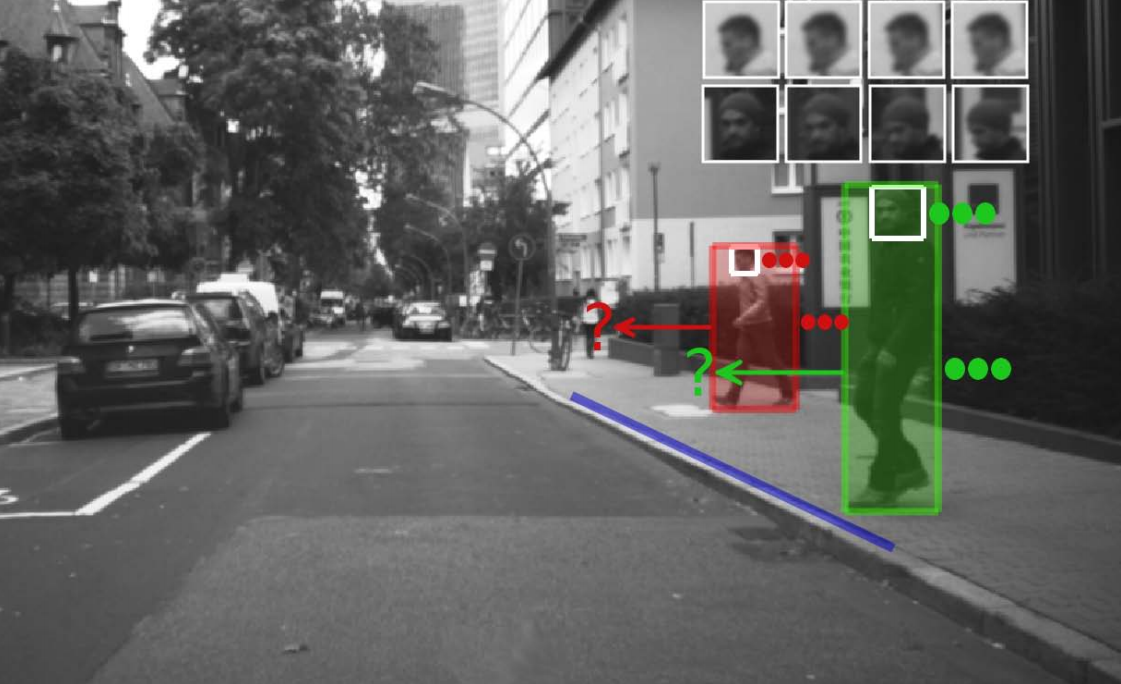
\includegraphics[width=\linewidth]{figures/motivaton.png}
  \caption{Pedestrian intent estimation~\cite{Kooij2018}. Humans are experts in estimating pedestrian intent, i.e. predicting whether the pedestrian is going to cross (red) or not (green). 
  Using computational models, our objective is to understand the underlying mechanism behind human decision making for pedestrian intent estimation.}
  \label{fig:overview}
\end{figure}